\section{Latent Dirichlet allocation}
The model is described as follows:
\begin{align}
    \vec \alpha                                 &\in (0, \infty)^T, \text{ usually} = \alpha\vec 1 \\
    \vec \gamma                                 &\in (0, \infty)^W, \text{ usually} = \gamma\vec 1 \\
    \vec \pi_d \given \vec \alpha               &\sim \Dir(\vec \alpha), d = 1, \dotsc, D \\
    \vec \beta_t \given \vec \gamma             &\sim \Dir(\vec \gamma), t = 1, \dotsc, T \\
    z_{n, d} \given \{\vec\pi_{\delta}\}        &\sim \Cat(\vec \pi_d), n = 1, \dotsc, N_d, d = 1, \dotsc, D \\
    w_{n, d} \given z_{n, d}, \{\vec \beta_t\}  &\sim \Cat\left(\vec \beta_{z_{n, d}}\right), n = 1, \dotsc, N_d, d = 1, \dotsc, D.
\end{align}
where we use the following indexing scheme:
\begin{itemize}
    \item $d$ or $\delta$ for document,
    \item $n$ or $\eta$ for word in a document,
    \item $t$ or $\tau$ for topic.
\end{itemize}
The graphical model can be seen in Figure~\ref{fig:models/lda/figures/lda} below.
\begin{figure}[htb!]
    \centering
        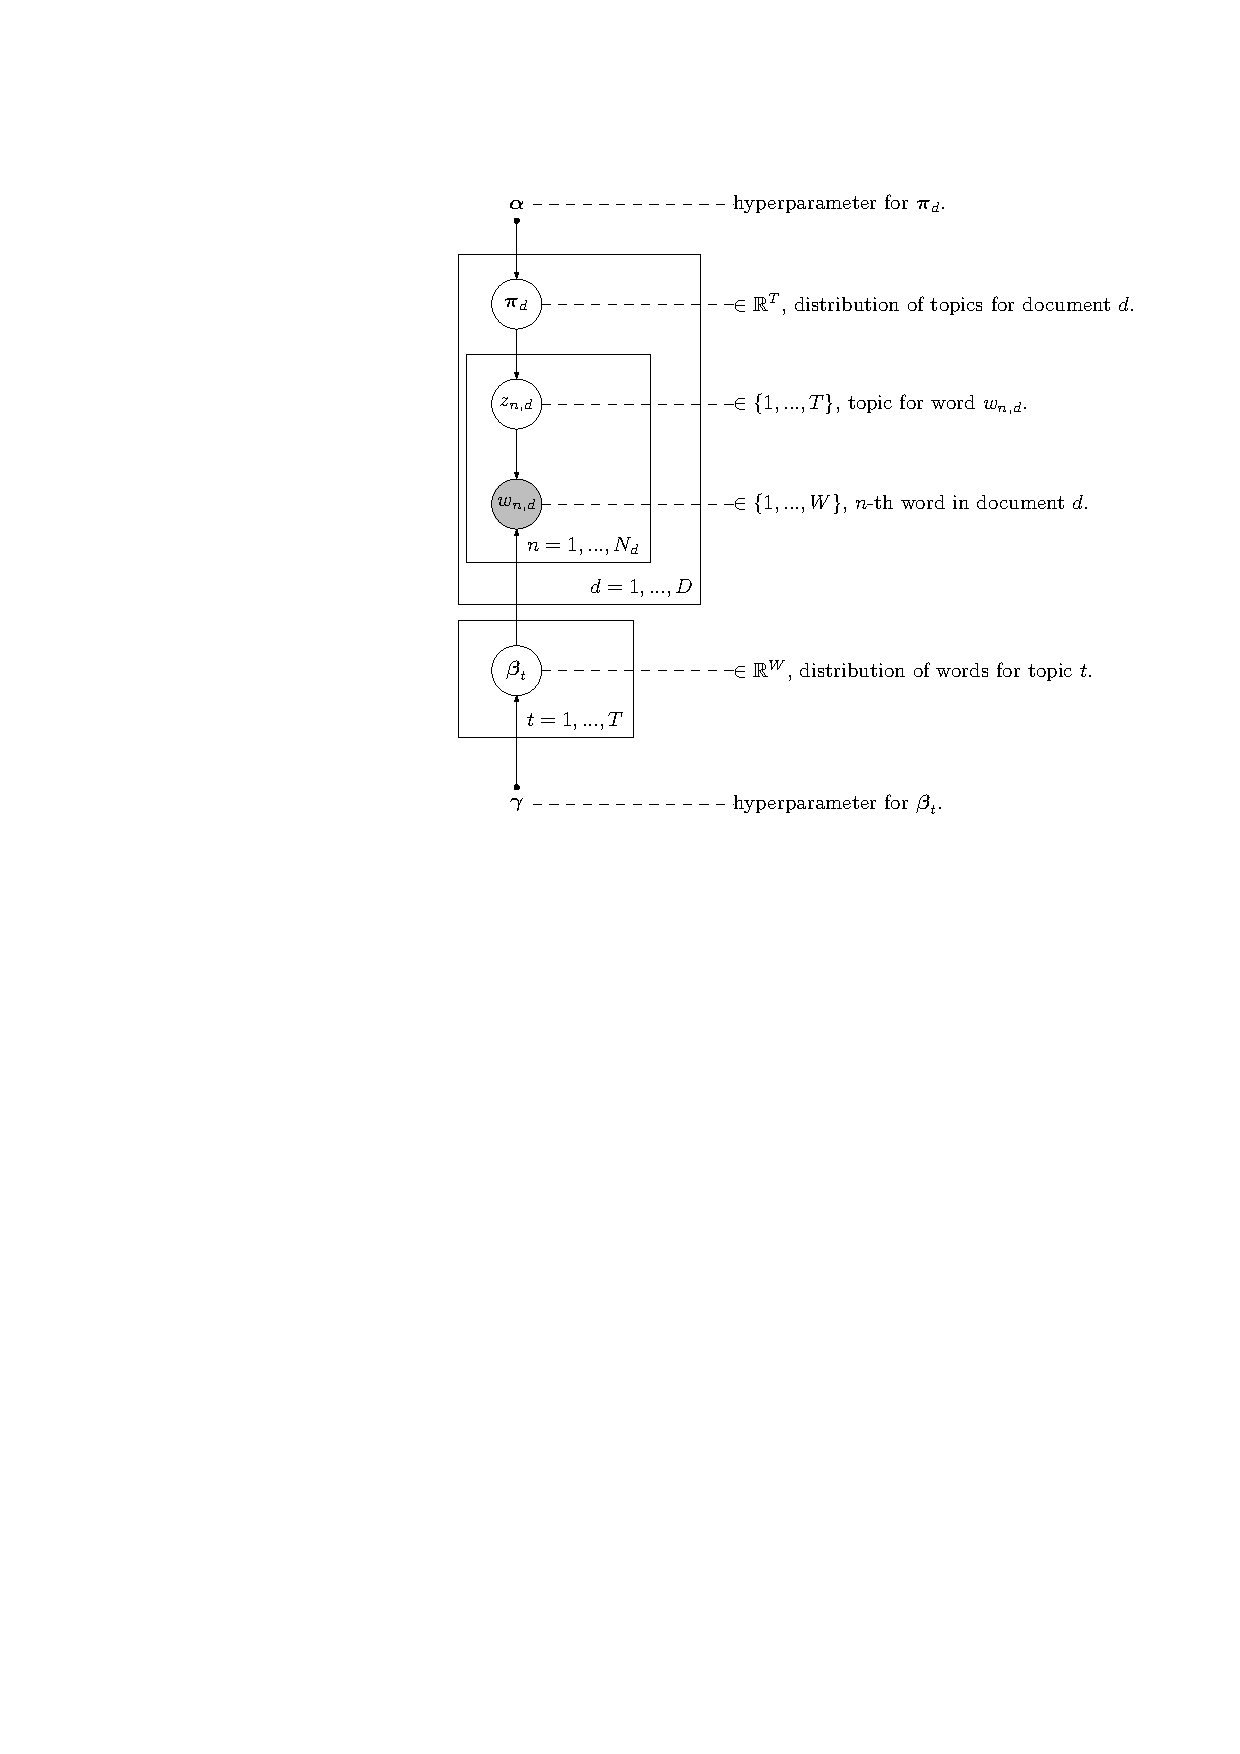
\includegraphics[width=0.5\textwidth]{models/lda/figures/lda}
    \label{fig:models/lda/figures/lda}
    \caption{Graphical model for Latent Dirichlet allocation.}
\end{figure}

The joint probability is
\begin{align}
    \hspace{2em}&\hspace{-2em}
    p\left(\{\vec \pi_d\}, \{z_{n, d}\}, \{w_{n, d}\}, \{\beta_t\} \given \vec \alpha, \vec \gamma\right) \\
    &= \left(\prod_d p(\vec \pi_d \given \vec \alpha)\right) \left(\prod_n \prod_d p(z_{n,d} \given \vec \pi_d)\right) \left(\prod_n \prod_d p(w_{n, d} \given z_{n, d}, \{\vec \beta_t\})\right) \left(\prod_t p(\vec \beta_t \given \vec \gamma)\right) \\
    &= \left(\prod_d \Dir(\vec \pi_d \given \vec \alpha)\right) \left(\prod_n \prod_d \Cat(z_{n, d} \given \vec \pi_d) \Cat(w_{n, d} \given \vec \beta_{z_{n, d}})\right) \left(\prod_t \Dir(\vec \beta_t \given \vec \gamma)\right)
\end{align}

\subsection{Gibbs sampling for LDA}
\subsection{Collapsed Gibbs sampling for LDA}